\chapter{معماری \lr{IMS}}
\label{archPart}
معماری \lr{IMS}، از سه لایه مختلف تشکیل می\nf شود که هر لایه، مستقل از سایر لایه\nf ها، وظایف مخصوص به خود را انجام می\nf دهد. پایین\nf ترین لایه که به آن سطح حامل و گاهاً سطح انتقال گفته می\nf شود، دارای منابع فیزیکیِ ضروی می\nf باشد. این منابع، برای ایجاد ارتباط و همچنین حمل \lr{payload}\RTLfootnote{بسته\nf های دیتا}(صدا و یا دیتا) بین نقطه\nf ی شروع و پایان ارتباط مورد استفاده قرار می\nf گیرند. لایه\nf ی میانی که به آن سطح کنترلی گفته می\nf شود، از یک سری المان هوشمند تشکیل شده است. این المان\nf ها، تعیین می\nf کنند که آیا کاربر، اجازه\nf ی استفاده از شبکه را دارد یا نه. همچنین این لایه، نحوه\nf ی مسیریابی تماس یا مسیر انتقال دیتا را تعیین می\nf کند که به این عمل، ایجاد جلسه\RTLfootnote{\lr{Session}} می\nf گویند. بالاترین لایه\nf ی این معماری که به آن سطح اپلیکیشن گفته می\nf شود، شامل تمام برنامه\nf ها و دیتای لازم برای ارائه سرویس به کاربر می\nf باشد. شکل \ref{arch}، المان\nf های معماری \lr{IMS} را در لایه\nf های مختلف و همچنین ارتباط آن\nf ها با یکدیگر را نشان می\nf دهد. در ادامه، این سه لایه به\nf طور خلاصه شرح داده شده\nf اند. مطالب این فصل، بر اساس \cite{blended} و \cite{3gims} نوشته شده\nf اند.

\begin{figure}[h]
\centering
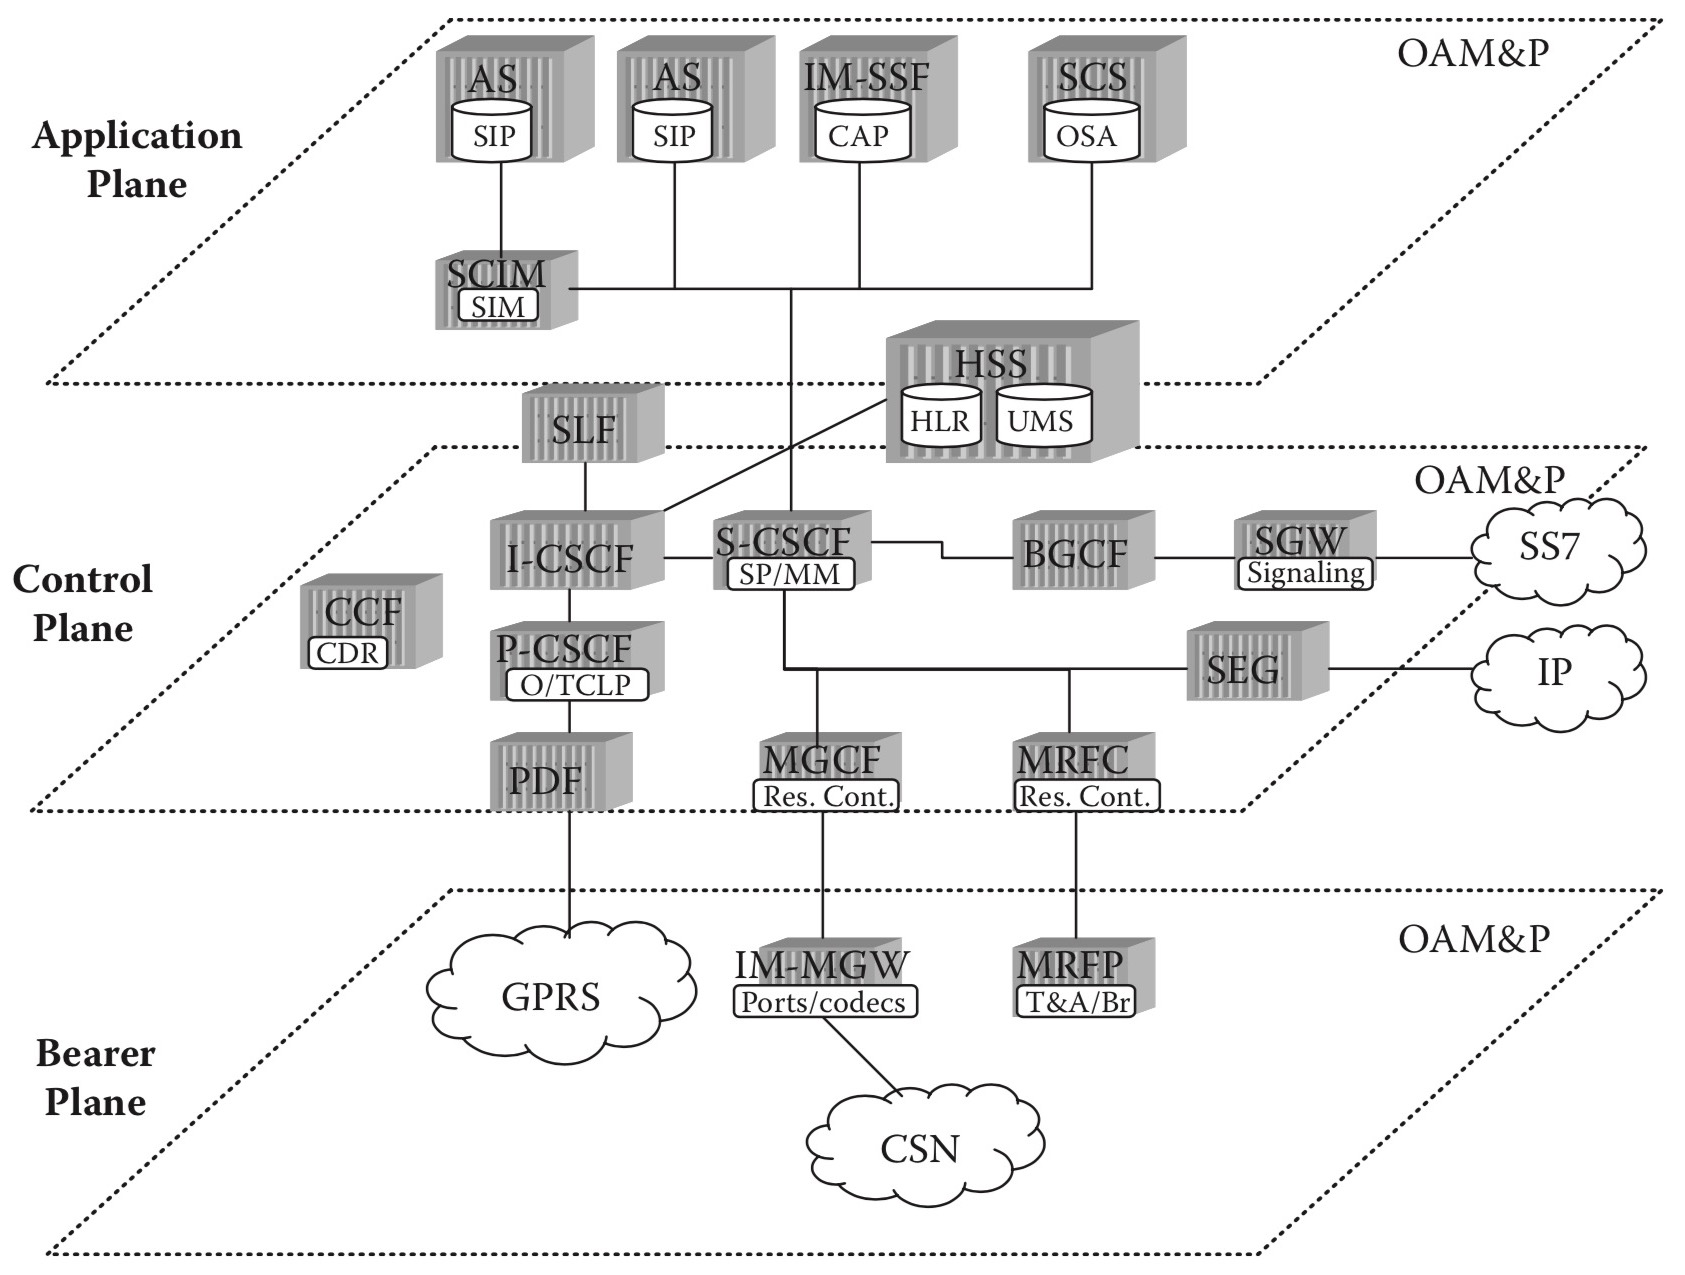
\includegraphics[width=\textwidth]{arch}
\caption{معماری لایه\nf ای شبکه\nf ی \lr{IMS}}
\label{arch}
\end{figure} 

\section{سطح کنترلی}
در \lr{IMS}، از آنجایی\nf که تمامی  سرویس\nf ها شامل پروتکل \lr{IP} هستند، کاربر به منظور فراخوانی هر یک از این سرویس\nf ها، نیاز به ایجاد یک جلسه دارد. سطح کنترلی، وظیفه\nf ی ایجاد این جلسات را دارد. به\nf طور کلی، سطح کنترلی از چهار المان اصلی تشکیل می\nf شود:
\begin{enumerate}
\begin{latin}
\item \textbf{CSCF}: Call Session Control Function(\rl{تابع کنترل جلسه\nf ی تماس})
\item \textbf{HSS}: Home Subscriber Server(\rl{سرور مرکزی مشترکین})
\item \textbf{BGCF}: Breakout Gateway Control Function(\rl{تابع کنترل درگاه خروجی}) 
\item \textbf{SGW}: Signaling Gateway(\rl{درگاه سیگنالینگ})
\end{latin}
\end{enumerate}

\subsubsection{CSCF}
المان \lr{CSCF}، پردازش تماس\nf ها و توابع کنترلی را فراهم می\nf کند و کاری مشابه سوئیچ\nf های مداری را انجام می\nf دهد. همچنین، از آنجایی\nf که \lr{IMS} یک شبکه\nf ی مبتنی بر \lr{IP} است، \lr{CSCF} توابع کنترل جلسه را نیز فراهم می\nf کند. استانداردها، \lr{CSCF} را به\nf عنوان یک سرور \lr{SIP}\RTLfootnote{سرواژه\nf ی عبارت \lr{Session Initiation Protocol} و به معنای پروتکل راه\nf اندزی جلسه} تعریف می\nf کنند که شامل سه جزء عملیاتی می\nf باشد:
\begin{itemize}
\item \lr{Proxy CSCF (P-CSCF)}
\end{itemize}

\indent این المان، نقطه\nf ی اوّلیه\nf ی ورود به معماری \lr{IMS} می\nf باشد،گرچه ممکن است که نقطه\nf ی اوّلیه\nf ی ورود برای کاربر نباشد. دستگاه کاربر\RTLfootnote{\lr{User Equipment(UE)}}، تمام پیام\nf های سیگنالینگ \lr{IMS} را به \lr{P-CSCF} می\nf فرستد. همچنین، عدم وابستگی \lr{IMS} به ناحیه\nf ی دسترسی توسّط این المان تأمین می\nf شود. \lr{P-CSCF} ممکن است که با \lr{PCRF}\RTLfootnote{سرواژه\nf ی عبارت \lr{Policy and Charging Rules Function} و به معنای تابع قوانین شارژ و سیاست } ادغام شود. \lr{PCRF}، وظیفه فراهم کردن کیفیت سرویس برای یک جلسه خاص را بر عهده دارد.


\begin{itemize}
\item \lr{Interrogating CSCF (I-CSCF)}
\end{itemize} 

\indent این المان، پیام\nf های فوروارد شده از \lr{P-CSCF} را دریافت می\nf کند و تعیین می\nf کند که دستگاه کاربر، به کدام \lr{S-CSCF} متّصل خواهدشد. \lr{I-CSCF}، پس از دریافت پیام ثبت\nf نام\RTLfootnote{\lr{Register}} از سمت دستگاه کاربر، از \lr{HSS} پرس\nf وجو می\nf کند که آیا این دستگاه، به یک \lr{S-CSCF} متّصل است یا خیر. در صورتی که این اتّصال وجود نداشته باشد،\lr{I-CSCF}، یک \lr{S-CSCF} به دستگاه کاربر اختصاص می\nf دهد. \lr{I-CSCF}، توپولوژی، پیکربندی و ظرفیت شبکه\nf ی اپراتور را از شبکه\nf های همتا مخفی نگه\nf می\nf دارد. این کار به\nf وسیله\nf ی تغییر و یا رمزکردن اطّلاعات حسّاس مانند نام دامنه و اطّلاعات مربوط به مسیریابیِ موجود در پیام\nf ها انجام می\nf شود.

\begin{itemize}
\item \lr{Serving CSCF (S-CSCF)}
\end{itemize} 

\indent این المان، در مرکز \lr{IMS} جای دارد و عمل پردازش تماس\nf ها را انجام می\nf دهد؛ درست مانند همان عملی که در سوئیچ\nf های مداری انجام می\nf شود. همچنین، پردازش سایر جلسات نیز بر عهده این المان می\nf باشد. تمام پیام\nf های \lr{SIP} که از دستگاه کاربر و یا به دستگاه کاربر ارسال می\nf شوند، از \lr{S-CSCF} می\nf گذرند. \lr{S-CSCF}، اطّلاعات وضعیت تمام جلسات دستگاه کاربر را نگه\nf می\nf دارد و بنابر موقعیّت، به\nf عنوان \lr{SIP proxy server} و یا \lr{SIP registrar} عمل می\nf کند.

\subsubsection{HSS}

المان \lr{HSS}،‌	 محل ذخیره دیتای پروفایل تمام مشترکین و همچینین اطّلاعات مربوط به احراز هویّت کاربران است. دیتای موقّتِ مربوط به مشترکین مانند وضعیت کنونی و مکان ثبت\nf نام آن\nf ها نیز در \lr{HSS} ذخیره میٖ\nf شود. \lr{HSS}، علاوه بر این که قادر به انجام تمام وظایف \lr{HLR}\RTLfootnote{سرواژه\nf ی عبارت \lr{Home Locatation Register}} است،‌	 باید قابلیت پشتیبانی از تمام وظایف مربوط به 	شبکه\nf های مبتنی بر \lr{IP} را نیز داشته باشد. \lr{HSS} برای برقراری ارتباط با سایر المان\nf های \lr{IMS} نظیر \lr{I/S-CSCF}، از پروتکل \lr{DIAMETER} استفاده می\nf کند. تشخیص هویّت،‌ تعیین اجازه\nf ی دسترسی و تأمین امنیّت اطّلاعات کاربران از کارکردهای اصلی \lr{HSS} هستند. به دلایل امنیتی، مقیاس\nf پذیری و  یا ایجاد افزونگی برای بالا بردن قابلیت اطمینان،‌ ممکن است از چند \lr{HSS} استفاده شود. در این صورت،‌ المان \lr{SLF}\RTLfootnote{سرواژه\nf ی عبارت \lr{Subscription Locator Function}} به معماری \lr{IMS} اضافه می\nf شود. این المان،‌ اطّلاعات لازم در مورد این که دیتای پروفایل کاربر در کدام \lr{HSS} قرار دارد را فراهم می\nf کند. 


\subsubsection{BGCF}

المان \lr{BGCF} مسئول تعیین نقطه\nf ی خروج\RTLfootnote{\lr{Breakout}} از شبکه\nf ی \lr{IMS}  به دامنه\nf ی سوئیچ مداری است. زمانی که \lr{S-CSCF} دیگر نمی\nf تواند مسیریابی جلسه را در شبکه\nf ی \lr{IMS} ادامه دهد(عموماً به این دلیل که نمی\nf تواند آدرس را از طریق  سرور نام دامنه به\nf دست آورد)، پیام\nf های \lr{SIP} را به \lr{BGCF} می\nf فرستد. المان \lr{BGCF} تشخیص می\nf دهد که آیا این خروج در درون همان شبکه یا در شبکه\nf ای دیگر رخ می\nf دهد. اگر این عمل مربوط به همان شبکه باشد، \lr{BGCF} یک \lr{MGCF}\RTLfootnote{سرواژه\nf ی عبارت \lr{Media Gateway Control Function} و به معنای تابع کنترل درگاه مدیا} را برای برقراری ارتباط بین\nf شبکه\nf ای با دامنه سوئچ مداری انتخاب می\nf کند. در صورتی که این خروج در شبکه\nf ی دیگری رخ دهد، \lr{BGCF} پیام\nf های سیگنالینگ جلسه را به \lr{BGCF} شبکه\nf ی مربوطه ارسال می\nf کند. در صورتی که شبکه\nf ی مقصد، فاقد المان \lr{BGCF} باشد(یعنی شبکه\nf ی مقصد \lr{IMS} را پیاده\nf سازی نکرده\nf باشد)، \lr{BGCF} این تماس را به شبکه\nf ی سوئیچ مداری خودش انتقال می\nf دهد\RTLfootnote{\lr{Hand Off}}. شبکه سوئیچ مداری نیز برقراری تماس را از طریق مسیریابی استاندارد \lr{PSTN}\RTLfootnote{سرواژه\nf ی عبارت \lr{Public Switched Telephone Network} و به معنای شبکه\nf ی سوئیچ عمومی تلفن} انجام می\nf دهد.


\subsubsection{SGW}
 
المان \lr{SGW} معمولاً به عنوان یکی از المان\nf های \lr{IMS} دیده نمی\nf شود زیرا عملکرد آن در لایه\nf های پایین\nf تر از لایه\nf ی \lr{SIP} است. المان \lr{SGW} می\nf تواند به\nf صورت مستقل و یا به\nf صورت یکپارچه با المان\nf های دیگر پیاده\nf سازی شود. این المان، عمل تبدیل سیگنالینگ\nf های لایه\nf ی انتقال را برای پیام\nf های سیگنالینگ کنترلی انجام می\nf دهد تا شبکه\nf های سیگنالینگ متفاوت را به یکدیگر متّصل کند.


\section{سطح حامل}

المان\nf های \lr{MGCF}\RTLfootnote{سرواژه\nf ی عبارت \lr{Media Gateway Control Function} و به معنای تابع کنترل درگاه مدیا} و \lr{MRFC}\RTLfootnote{سرواژه\nf ی عبارت \lr{Media Resource Function Controller} و به معنای کنترل کننده\nf ی تابع منابع مدیا} در سطح کنترلی قرار دارند، امّا از آنجایی\nf که این دو المان، ارتباط تنگاتنگی با یکی از المان\nf های اصلی سطح حامل به نام \lr{IMS-MGW}\RTLfootnote{کوتاه\nf شده\nf ی عبارت \lr{IMS Media Gateway} و به معنای درگاه مدیای \lr{IMS}} دارند، این دو المان در این بخش مورد بحث قرار گرفته\nf اند.


\subsubsection{رابطه\nf ی \lr{IMS-MGW} و \lr{MGCF}}

هر زمان که یک کاربر در دامنه\nf ی سوئیچ مداری بخواهد با یک کاربر در دامنه\nf ی سوئیچ بسته\nf ای ارتباط برقرار کند، باید عمل تبدیل بین حامل\nf های مداری و بسته\nf ای صورت گیرد. المان \lr{MGCF} مسئول تبدیل سیگنال\nf های کنترلی تماس تلفن ثابت و \lr{SIP} به یکدیگر است. در انجام این کار، \lr{MGCF} عمل \lr{binding} بین شناسه\nf های سطح حامل \lr{IP} و شناسه\nf های سطح حامل سوئيچ مداری را انجام می\nf دهد. المان \lr{MGCF} باید این اطّلاعات را با \lr{IMS-MGW} مبادله کند تا تماس بتواند از طریق \lr{IMS-MGW} برقرار شود(شکل\ref{bearer1}). همچنین، به دلیل این\nf که روش\nf های کدگذاری زیادی برای جلسات صوتی و تصویری وجود دارد، \lr{IMS-MGW} باید بداند که از کدام یک از این روش ها استفاده شده است.

\begin{figure}[h]
\centering
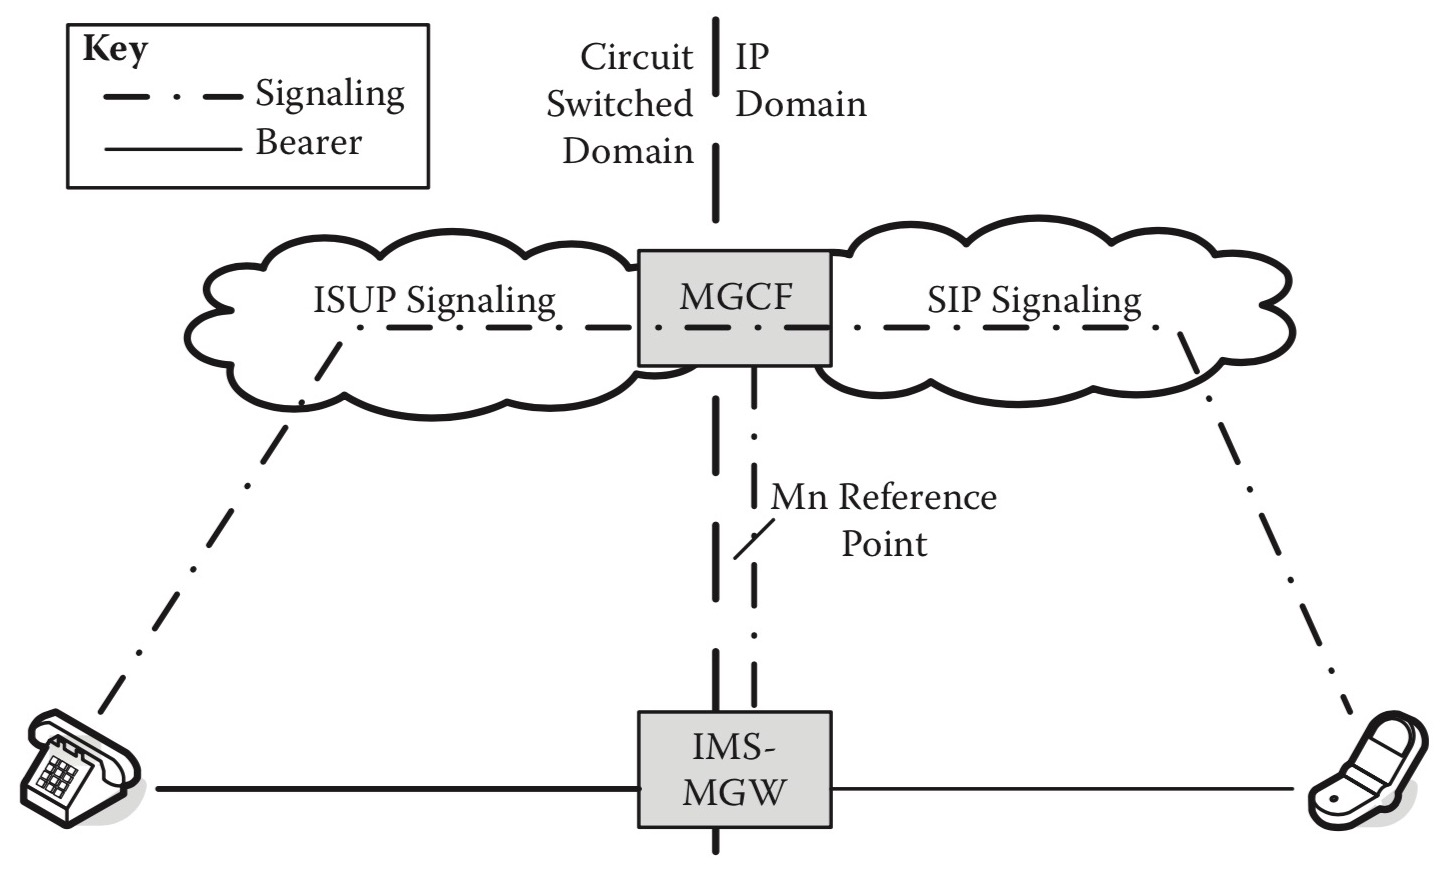
\includegraphics[width=\textwidth]{bearer1}
\caption{ارتباط بین \lr{IMS-MGW} و \lr{MGCF}}
\label{bearer1}
\end{figure} 

\subsubsection{ارتباط بین \lr{MRFP} و \lr{MRFC}}

المان \lr{MRFC} در واقع کنترل\nf کننده\nf ی المان \lr{MRFP}\RTLfootnote{سرواژه\nf ی عبارت \lr{Multimedia Resource Function Controller Processor} و به معنای پردازند\nf ی \lr{MRFC}} و رابط بین \lr{MRFP} و \lr{CSCF} است(شکل\ref{bearer2}). ارتباط بین المان  \lr{MRFC} و \lr{CSCF} از طریق پروتکل \lr{SIP} انجام می\nf شود. المان \lr{MRFP} مسئول انجام وظایف زیر است:

\begin{figure}[h]
\centering
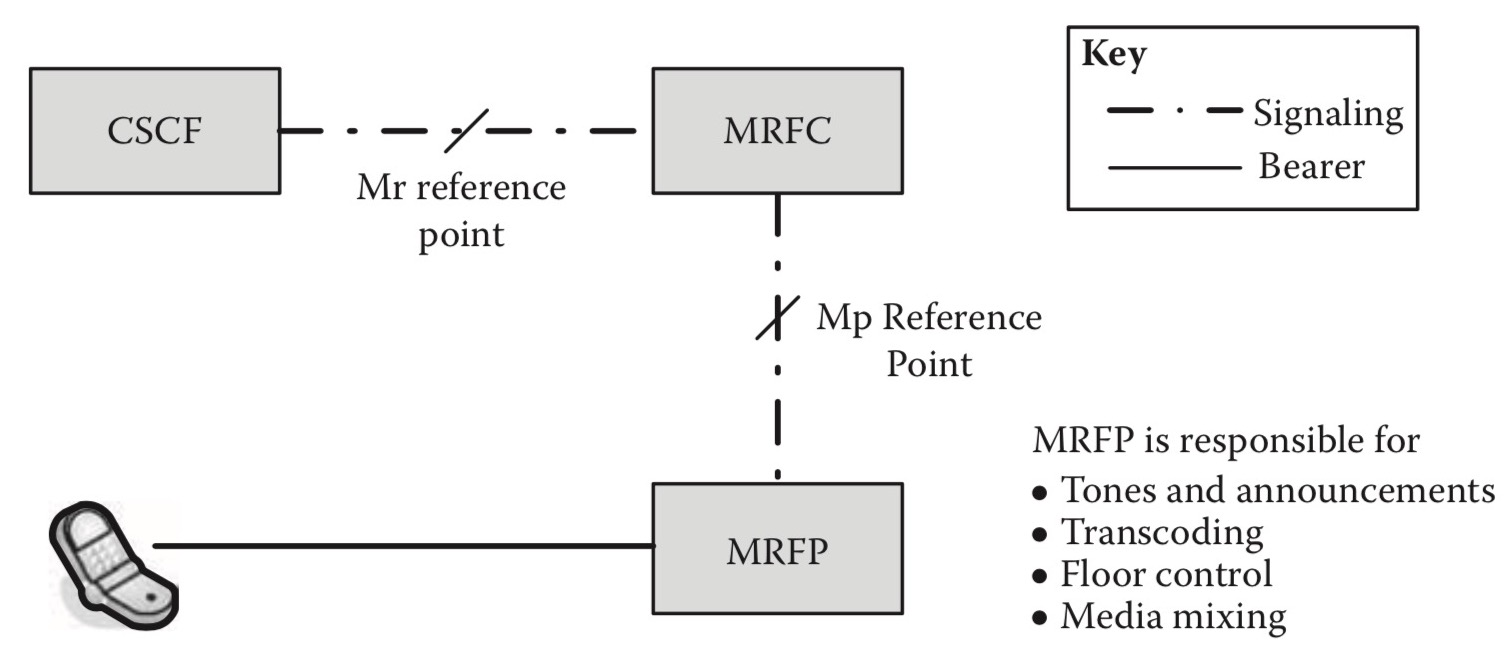
\includegraphics[width=\textwidth]{bearer2}
\caption{ارتباط بین \lr{MRFP} و \lr{MRFC}}
\label{bearer2}
\end{figure}
\begin{itemize}
\item آهنگ\nf ها و اعلان\nf ها

پخش صدای بوق آزاد و یا اشغال در هنگام تماس و یا پخش آهنگ پیشواز و همچنین پخش اعلان\nf هایی مانند: مشترک مورد نظر در دسترس نمی\nf باشد.
\newline
\\
\item تبدیل کدگذاری\nf ها

\lr{IMS}، روش کدگذاری را در هنگام ایجاد جلسه انتخاب می\nf کند و هیچ تضمینی وجود ندارد که دو طرف مکالمه از روش کدگذاری یکسان استفاده کنند. لذا نیاز است که فرآیند تبدیل بین کدگذاری\nf ها انجام شود.
\item کنترل بستر

کنترل بستر، برای انجام مکالماتی که در هر لحظه، فقط یک نفر قادر به ارسال اطّلاعات است، ضروری می\nf باشد. شخصی که در هر لحظه، بستر را در اختیار دارد، تنها کسی است که می\nf تواند اطّلاعاتی مانند صوت را ارسال کند و مابقی شرکت\nf کننده\nf ها در آن جلسه، فقط صدای آن فرد را می\nf شنوند. در سرویس\nf هایی که اطّلاعت ویدیوئی ارسال می\nf کنند نیز، تنها تصویر شخصی که بستر را در اختیار دارد، برای سایر افراد نمایش داده می\nf شود. سرویس \RTLfootnote{سرواژه\nf ی عبارت \lr{Push to Talk Over Cellular}}PoC و \RTLfootnote{سرواژه\nf ی عبارت \lr{Push To Video}}PTV، از جمله سرویس\nf هایی هستند که به کنترل بستر نیازمند می\nf باشند.

\item درهم آمیختن مدیا

درهم آمیختن مدیا، برای انجام کنفرانس\nf های صوتی و یا ویدیوئی در بستر \lr{IMS} مورد استفاده قرار میگیرد. شرکت\nf کننده\nf ها در کنفرانس\nf های صوتی، ترکیبی از صدای سایر شرکت\nf کننده\nf ها را می\nf شنوند. در کنفرانس ویدوئی نیز صفحه نمایش به بخش\nf های مختلف تقسیم شده و هر بخش، تصویر یک شرکت\nf کننده در کنفرانس را نمایش می\nf دهد.
\end{itemize}


\section{سطح اپلیکیشن}
اپرواتورها می\nf توانند با استفاده از سطح اپلیکیشن، اپلیکیشن\nf های نوظهور و یا اپلیکیشن\nf های ترکیبی را در اختیار کاربران قرار دهند. به اپلیکیشن\nf هایی که قابلیت ترکیب شدن با اپلیکیشن\nf های فعلی، دستگاه\nf ها و منابع محتوا را دارند و می\nf توانند با این کار، سرویسی با ارزش\nf تر را برای کاربران فراهم کنند، اپلیکیشن\nf های ترکیبی گفته می\nf شود. اپلیکیشن\nf های فعلی می\nf توانند اپلیکیشن\nf هایی از دنیای اینترنت و یا اپلیکیشن\nf هایی باشند که اپرواتور آن\nf ها را از قبل پیاده\nf سازی کرده است. المان\nf های شبکه\nf ای که سطح اپلیکیشن را تشکیل می\nf دهند، عموماً به \lr{S-CSCF} و \lr{HSS} متّصل می\nf شوند. 
\begin{figure}[h]
\centering
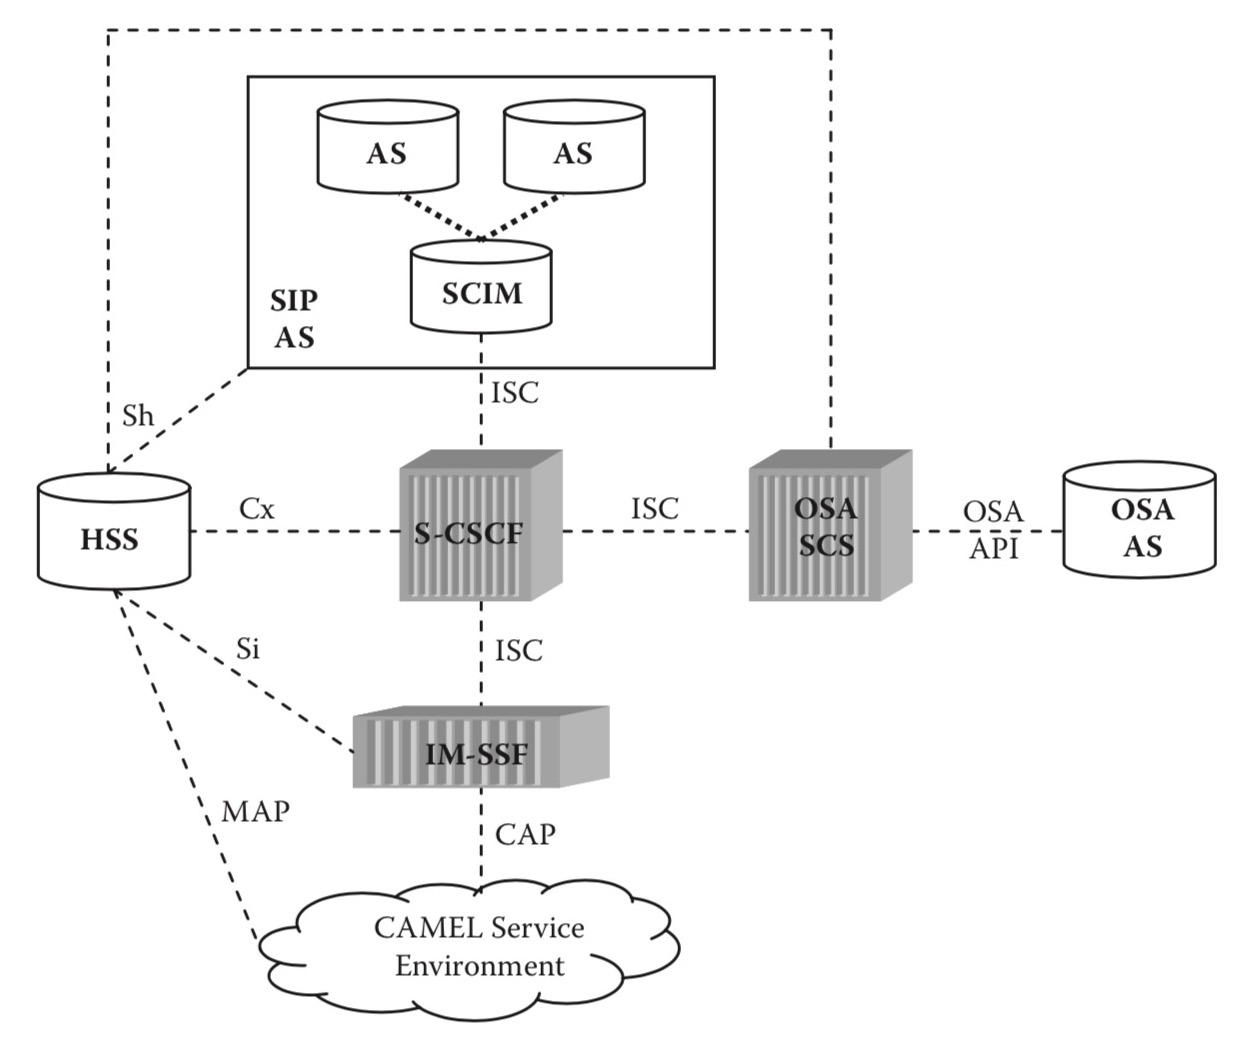
\includegraphics[width=\textwidth]{asref}
\caption{معماری لایه\nf ی اپلیکیشن و ارتباط این لایه با سایر المان\nf های \lr{IMS}}
\label{asref}
\end{figure}
\subsubsection{اپلیکیشن سرورهای \lr{SIP}}

اپلیکیشن\nf های \lr{IMS} به\nf طور عمده به\nf وسیله\nf ی اپلیکیشن سرورهای برمبنای \lr{SIP} پیاده\nf سازی شده\nf اند. کاربر، با فراخوانی این اپلیکیشن سرورها، از خدمات اپراتور بهره\nf مند می\nf شود. طبق استانداردها، \lr{IMS} باید بتواند جلسه\nf ای را ایجاد کند که در آن، به\nf طور هم\nf زمان از چند اپلیکیشن سرور استفاده می\nf شود. این امکان وجود دارد که پاسخ و خرجی یک اپلیکیشن سرور، به\nf عنوان ورودی اپلیکیشن سرور دیگر مورد استفاده قرار گیرد یا این که پس از فراخوانی یک اپلیکیشن سرور، نیاز به فراخوانی اپلیکیشن سرور بعدی نباشد. بنابراین باید مکانیزمی وجود داشته باشد که اپلیکیشن سرور(های) مناسب را برای کاربر انتخاب کند و همچنین ترتیب فراخوانی اپلیکشن سرورها را نیز کنترل کند.

المان \lr{HSS} در پروفایل دیتای مشترکین، لیستی از اپلیکیشن سرورهای مختص ِهر کاربر و ترتیب فراخوانی آن\nf ها را ذخیره می\nf کند. این لیست که \lr{iFC}\RTLfootnote{سرواژه\nf ی عبارت \lr{initial Factor Criteria} و به معنای معیارهای فاکتور اوّلیه} نام دارد، در طول فرایند ثبت\nf نام، با \lr{S-CSCF} به اشتراک گذاشته می\nf شود. محتوای کلی \lr{iFC} که از \lr{HSS} به \lr{S-CSCF} فرستاده می\nf شود، شامل موارد زیر است:


\begin{itemize}
\item آدرس اپلیکیشن سرور
\item اولویّت اپلیکیشن سرور(ترتیب فراخوانی)
\item اطّلاعات اختیاری مربوط به سرویس
\item نقطه\nf ی راه\nf اندازی\RTLfootnote{نقطه\nf ی راه\nf اندازی تعیین می\nf کند که چه زمانی \lr{iFC} فراخوانی شود}
\end{itemize}

\begin{figure}[h]
\centering
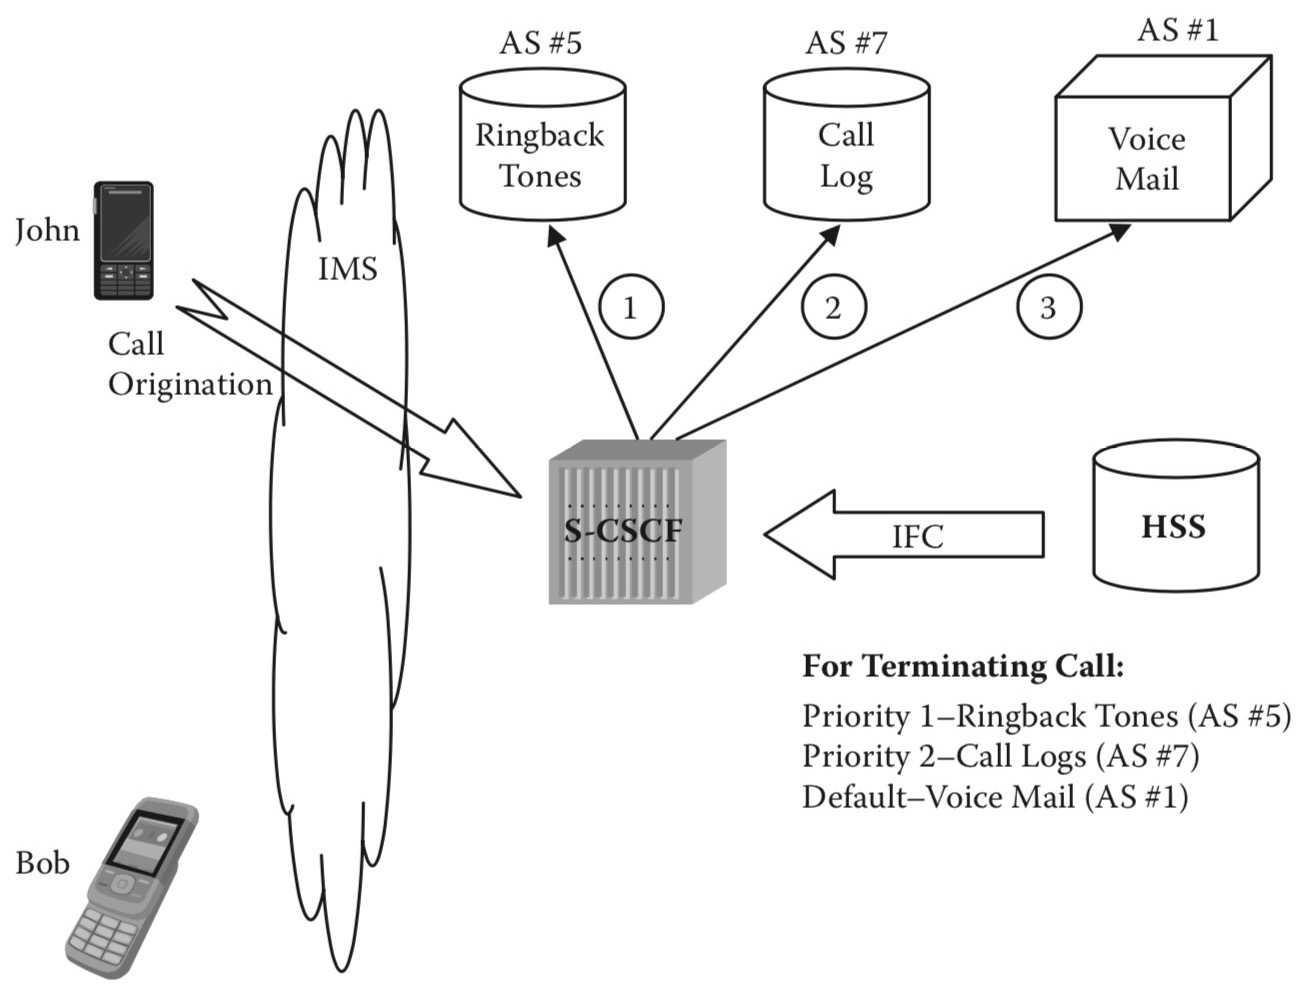
\includegraphics[scale=.25]{ifc}
\caption{مثال از ترتیب فراخوانی اپلیکیشن سرورها و کارکرد \lr{iFC}}
\label{ifc}
\end{figure}

در شکل \ref{ifc}، اهمیّت ترتیب فراخوانی اپلیکیشن سرورها و همچنین کاربرد \lr{iFC}، به\nf وسیله\nf ی یک مثال نشان داده شده است. در مثال شکل \ref{ifc}، تلفن همراه \lr{Bob} یک تماس از تلفن همراه \lr{John} دریافت می\nf کند. المان \lr{S-CSCF} به لیست دریافت\nf شده از \lr{HSS} نگاه می\nf کند و اپلیکیشن سرور شماره ۵ را فراخوانی می\nf کند و \lr{John} صدای بوق تماس \lr{Bob} یا آهنگ پیشواز او را می\nf شنود. از آنجایی\nf که \lr{Bob} می\nf خواهد سوابق تماس\nf های خود را ثبت کند و نگه\nf دارد، اپلیکیشن سرور شماره ۷ فراخوانی می\nf شود. در آخر نیز، چون \lr{Bob} مشغول انجام کاری است و نمی\nf خواهد تلفن \lr{John} را جواب بدهد، عملی که به صورت پیش\nf فرض در نظر گرفته\nf شده انجام می\nf شود؛ یعنی اپلیکیشن سرور شماره ۱ فراخوانی شده و تماس به صندوق پست صوتی منتقل می\nf شود. در شکل \ref{ifc}، ترتیب فراخوانی اپلیکیشن سرورها به\nf وسیله\nf ی عددی بر روی پیکان\nf ها مشخّص شده است. 

\subsubsection{\lr{IM-SSF}}
المان \lr{IM-SSF}\RTLfootnote{سرواژه\nf ی عبارت \lr{IP Multimedia Service Switching Function} و به معنای عملگر سرویس سوئیچینگ چندرسانه\nf ای \lr{IP}}، طرّاحی شده است تا اپراتورهای تلفن همراه را قادر سازد که از تکنولوژی \lr{GSM} کنونی خود یا زیرساخت اپلیکشن \lr{2G}، در کنار \lr{IMS} استفاده کنند. با استفاده از \lr{IM-SSF}، نیازی به صرف هزینه\nf ی بالا برای توسعه و پیاده\nf سازی دوباره\nf ی این اپلیکیشن\nf ها نیست. برای مثال، روش\nf های متنوّعی که برای خرید سرویس\nf های متنوّع از اپراتور وجود دارد(مثلاً خرید بسته اینترنت یا خرید بسته\nf ی ترکیبی اینترنت و پیام کوتاه) قبلاً توسّط اپراتور در \lr{GSM} پیاده\nf سازی شده\nf اند. در صورتی که این اپراتور بخواهد از \lr{IMS} استفاده کند دیگر نیاز نیست اپلیکشن مربوطه را دوباره و منطبق با معماری \lr{IMS} طرّاحی و پیاده\nf سازی کند و می\nf تواند از همان اپلیکیشنِ قبلی خود استفاده کند.


مطابق شکل \ref{asref}، \lr{IM-SSF} پیام\nf های \lr{SIP} را از \lr{S-CSCF} دریافت می\nf کند و آن\nf ها را به پیام\nf های معادل در \lr{CAMEL}\RTLfootnote{سرواژه\nf ی عبارت \lr{Customized Application for Mobile Netwrok Enhanced Logic}} ترجمه می\nf کند. لذا، \lr{IM-SSF} از طرف المان \lr{S-CSCF} به عنوان یک اپلیکیشن سرور دیده می\nf شود. از آنجایی\nf که استاندارد  \lr{IMS} توسّط \lr{3gpp} توسعه یافته است، طبیعی است که آن\nf ها مکانیزمی را درنظر گرفته\nf اند که \lr{IMS} با سیستم\nf های پیشین(که بر اساس استاندارد \lr{3gpp} طرّاحی شده\nf اند) تعامل داشته باشد.


\subsubsection{درگاه \lr{OSA}}
\label{osapart}

درگاه \lr{OSA}، ارتباط بین شبکه\nf ی داخلی اپراتور و شرکت\nf های شخص ثالث را برقرار می\nf کند تا این شرکت\nf ها بتوانند با استفاده از زیرساخت اپراتور مربوطه، سرویس خاصی را به مشترکین آن اپراتور ارائه دهند. می\nf توان گفت که \lr{OSA}، تسهیل\nf کننده\nf ی ورود سایر شرکت\nf ها، خصوصاً شرکت\nf های کوچک و استارت\nf آپ\nf های نوپا به بازار مخابرات است. المان \lr{OSA}، علاوه بر نقشی که به\nf عنوان رابط دارد، وظیفه ایجاد امنیّت و مدیریّت شارژ حساب کاربران را نیز  برعهده دارد\RTLfootnote{این کار را برای شرکت\nf های شخص ثالث انجام می\nf دهد}. رابطی که درگاه \lr{OSA} را به اپلیکیشن شرکت شخص ثالث متصّل می\nf کند، \lr{Parlay} نام دارد. از آنجایی\nf که سرویس\nf های شرکت\nf های شخص ثالث، عمدتاً به صورت اپلیکیشن\nf های مبتنی بر وب عرضه می\nf شوند، یک نسخه\nf ی مبتنی بر سرویس وب از  این رابط به نام \lr{Parlay X} طرّاحی شده است. رابط \lr{Parlay X}، توسعه\nf دهندگان اینترنت و اپلیکیشن\nf های تحتِ وب  را قادر می\nf سازد که بدون نیاز به یادگیری رابط \lr{Parlay} و قواعد پیچیده\nf ی آن، اپلیکیشن خود را متناسب با زیرساخت اپراتور طرّاحی کنند. 


شکل \ref{archref}، یک نمای کلّی از معماری \lr{IMS} را نشان می\nf دهد. در این فصل، بیشتر المان\nf ها و رابط\nf های موجود بین المان\nf های این معماری به\nf طور خلاصه بیان شد. برخی از بخش\nf های معماری \lr{IMS} نیز در فصل\nf های بعد توضیح داده شده\nf اند.
\begin{figure}[h]
\centering
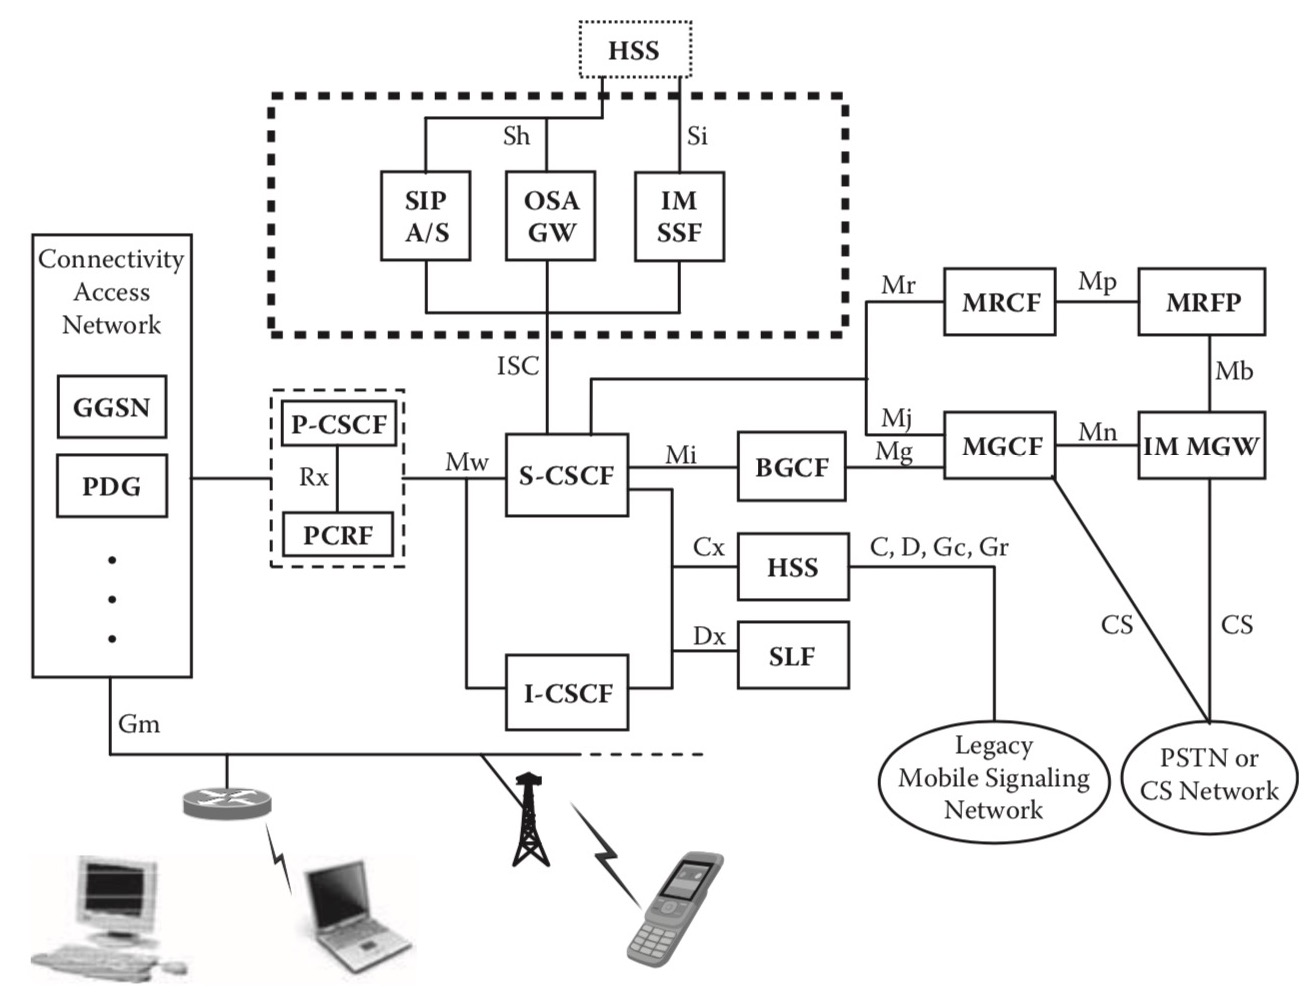
\includegraphics[width=\textwidth]{archref}
\caption{معماری مرجع برای \lr{IMS}}
\label{archref}
\end{figure}

